\begin{figure*}[ht!]
\centering
	\begin{subfigure}{0.33\textwidth}
                \centering
		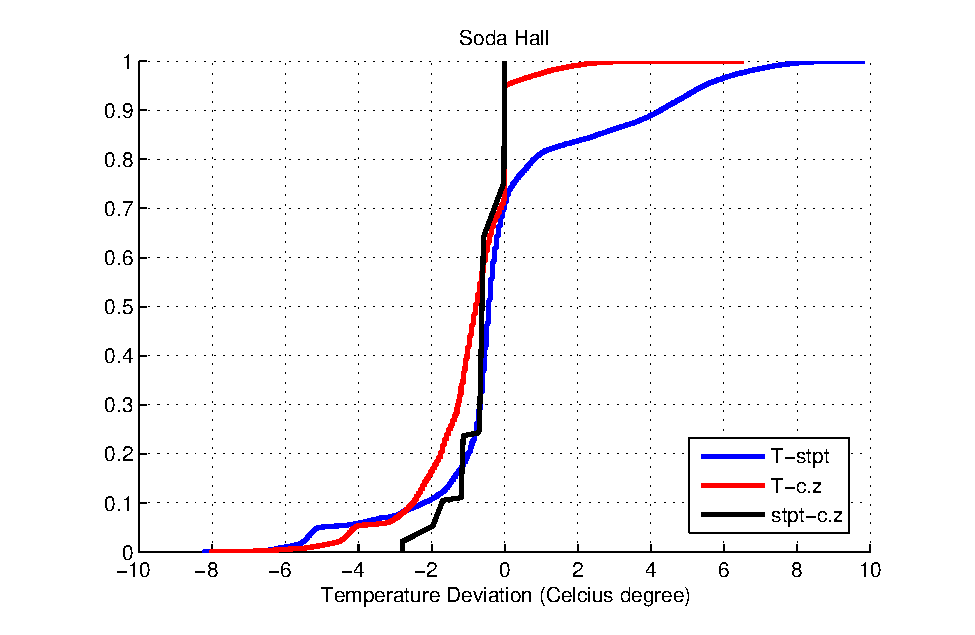
\includegraphics[width=\textwidth]{./figs/Soda_new.eps}
                \caption{Building A}
	\end{subfigure}
	\begin{subfigure}{0.33\textwidth}
                \centering
		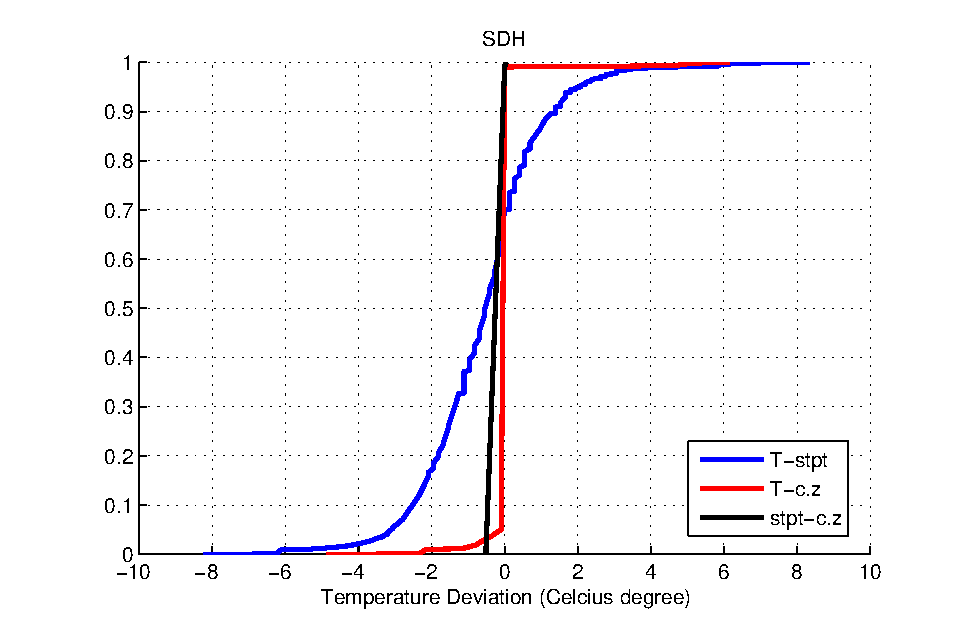
\includegraphics[width=\textwidth]{./figs/SDH_new.eps}
                \caption{Building B}
	\end{subfigure}
	\begin{subfigure}{0.33\textwidth}
                \centering
		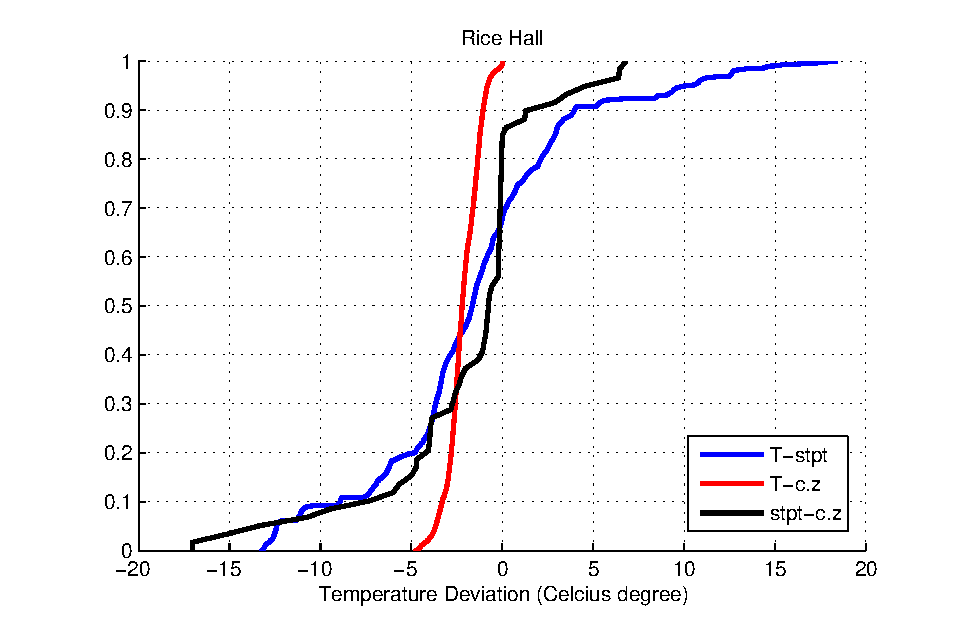
\includegraphics[width=\textwidth]{./figs/Rice_new.eps}
                \caption{Building C}
	\end{subfigure}
\caption{For each building, we present the distribution of temperature deviation between: a) room temperature and the corresponding setpoint, b) room temperature and the comfort range suggested by ASHRAE, c) room temperature setpoint and the ASHARE comfort suggestion. }
\label{fig:cdf_temp}
\end{figure*}

\section{Case Study}
In this section, we demonstrate that, with the metadata automatically normalized and generated using the techniques in previous section, we are able to implement a few applications that are generalizable from one building to another building without modification.

\subsection{Experimental Setup}
We implement \# applications and perform the analysis on three buildings from two campuses, and each building is installed with a different management system. Building A was built in mid-1990s using the system from Barrington ~\cite{}. Building B was recently built in 2005 using the Siements BACnet system~\cite{}. Building C is the newest building among the three using Trane's system~\cite{}, which was put into use from 2011. We collected all the available data readings from each building, covering temperature, humidity, co2 concentration, light intensity, air damper and valve postions, air volume, setpoints for various streams. The data used from each building was one-week data in June 2009, January 2012 and June 2013 respectively.
\subsection{Uncomfortable Rooms}
